% 1977 年江苏连云港市初试卷第 8 题：⊙O 中弦 AD、直径 AC，
% 半径 OH⊥AD 交 AD 于 B，求 BC 的长（按源卷第 3 页「第八题」布局，AB=BD=4、OB=3、半径=5 等比例缩放）
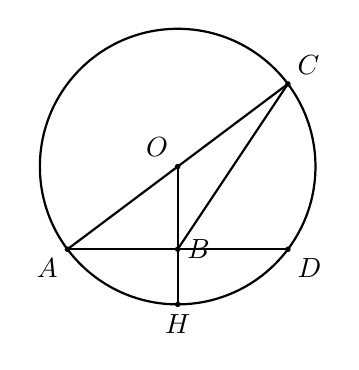
\begin{tikzpicture}[scale=1]
  \coordinate (O) at (0,0);
  \coordinate (A) at (-1.4,-1.05);
  \coordinate (D) at (1.4,-1.05);
  \coordinate (H) at (0,-1.75);
  \coordinate (C) at (1.4,1.05);
  \coordinate (B) at (0,-1.05);
  \draw[thick] (O) circle (1.75);
  \draw[thick] (A) -- (D);
  \draw[thick] (A) -- (C);
  \draw[thick] (O) -- (H);
  \draw[thick] (B) -- (C);
  \fill (O) circle (1pt) node[above left] {$O$};
  \fill (A) circle (1pt) node[below left] {$A$};
  \fill (D) circle (1pt) node[below right] {$D$};
  \fill (H) circle (1pt) node[below] {$H$};
  \fill (C) circle (1pt) node[above right] {$C$};
  \fill (B) circle (1pt) node[right] {$B$};
\end{tikzpicture}
